\documentclass[12pt]{article}
\usepackage{geometry}                % See geometry.pdf to learn the layout options. There are lots.
\geometry{letterpaper}                   % ... or a4paper or a5paper or ... 
%\geometry{landscape}                % Activate for for rotated page geometry
\usepackage[parfill]{parskip}    % Activate to begin paragraphs with an empty line rather than an indent
\usepackage{daves,fancyhdr,natbib,graphicx,dcolumn,amsmath,lastpage,url}
\usepackage{amsmath,amssymb,epstopdf,longtable}
\usepackage{paralist} 
\usepackage[final]{pdfpages}
\DeclareGraphicsRule{.tif}{png}{.png}{`convert #1 `dirname #1`/`basename #1 .tif`.png}
\pagestyle{fancy}
\lhead{CE 3372 -- Water Systems Design}
\rhead{SPRING 2025}
%\rhead{SPRING 2016}
%\rhead{FALL 2011}
%\rhead{SPRING 2012}
%\rhead{FALL 2012}
%\rhead{FALL 2015}
%\rhead{FALL 2010}
%\lfoot{EXERCISE 1 -- REVISION 1}
%\lfoot{EXERCISE 1 -- REVISION 2}
%\lfoot{EXERCISE 1 -- REVISION 3}
%\lfoot{EXERCISE 1 -- DUE 26 JAN 2012}
%\lfoot{EXERCISE 1 -- DUE 4 SEP 2012}
\lfoot{EXERCISE 5}
\cfoot{}
\rfoot{Page \thepage\ of \pageref{LastPage}}
\renewcommand\headrulewidth{0pt}
\newcommand\tab[1][1cm]{\hspace*{#1}}


\begin{document}
\begin{center}
\textbf{MEMORANDUM}
%{\textbf{{ CE 3372 -- Water Systems Design} \\ {Exercise Set 2}}}
\end{center}
\begingroup
\begin{tabular}{p{1in} p{5in}}
To: & P. N Guin \\ ~\\
From: & P. Olar Bear \\ ~\\
Date: & 04JAN2024 \\ ~\\
Subject: & CE 3372 -- Water Systems Design, Exercise Set 5. ~\\
\end{tabular}
\endgroup

\section*{\small{Problem 1}}  
This memorandum presents an analysis of a water transfer system that lifts water from one elevation to another.

\section*{\small{Discussion}}
The solution applies the energy equation and pumping concepts, computes a system curve, and uses that curve to find an operating point.
The remainder of this section presents the various steps required, with intermediate calculations shown and references imbedded into the memorandum.
The results for each problem are presented in the narrative below; the by-hand analysis is attached to this memorandum.

%%%%%%%%%%%%%%%%%%%%%%%%%%%%%%%%%%%%%%%%%%%%%%%%%%%%%%%%
\begin{enumerate}[a)]
\item A sketch of the water supply system that draws from a river at an elevation of 800-feet and delivers the water to a storage reservoir at elevation 820-feet s shown in Figure \ref{fig:SystemSchematic}.  On the figure, the supply pipeline, which is a 1000-foot long, 10-inch diameter, cast iron pipe, is labeled.  The single pump follows the performance curve shown below on Figure \ref{fig:PumpCurve2}.
\begin{figure}[h!] %  figure placement: here, top, bottom, or page
\centering
   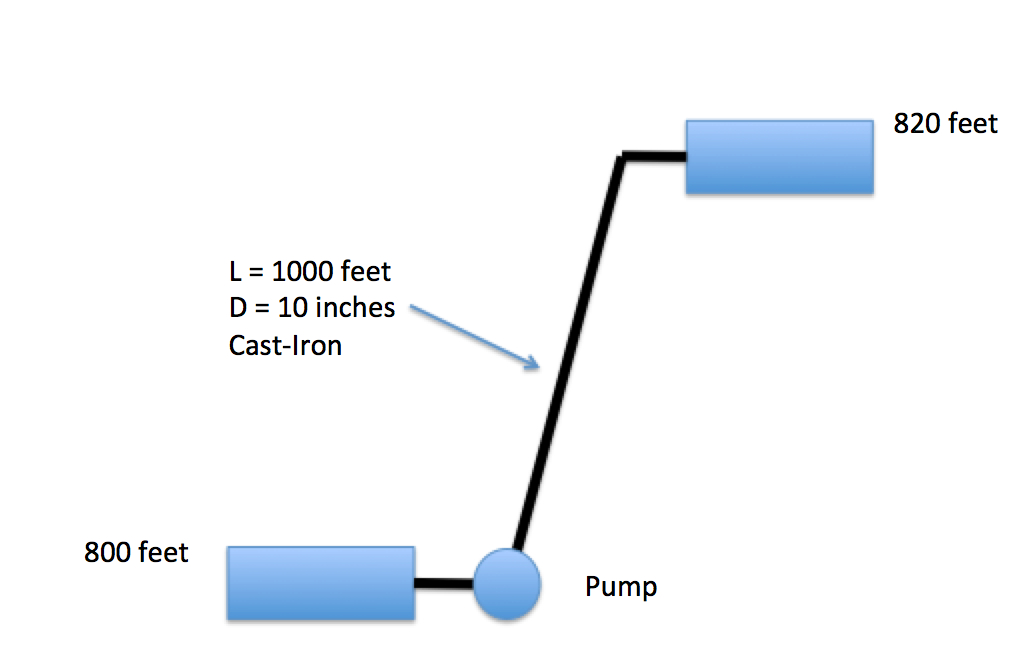
\includegraphics[width=5in]{SystemSchematic.jpg}
   \caption{Sketch of the system}
   \label{fig:SystemSchematic} 
\end{figure}

\item The inlet and outlet minor loss coefficients are 0.5 for the inlet (assumed flush, not re-entrant) and 1.0 for the outlet (small diameter into essentially infinite diameter pool).  
The values are obtained from directly Figure \ref{fig:LossCoefficients} below.
\begin{figure}[h!] %  figure placement: here, top, bottom, or page
\centering
   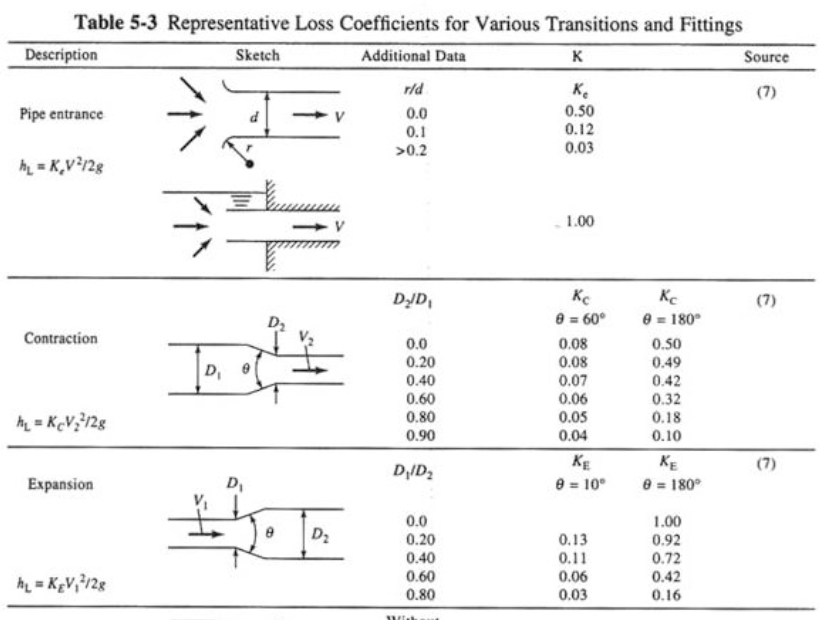
\includegraphics[width=4in]{LossCoefficients.jpg}
   \caption{Loss Coefficients from Fluid Mechanics Textbook \newline (p 381 in DF Elger, BC Williams, Crowe, CT and JA Roberson, Engineering Fluid Mechanics 10th edition, John
Wiley \& Sons, Inc., 2013.)}
   \label{fig:LossCoefficients} 
\end{figure}
\item The roughness ratio for use in the Moody chart for cast-iron pipe is 
\begin{equation}
\frac{k_s}{D} = \frac{0.00085}{10/12} = 0.00102
\end{equation}
The values are taken directly from Figure \ref{fig:RoughnessHeights} below.
\begin{figure}[h!] %  figure placement: here, top, bottom, or page
\centering
   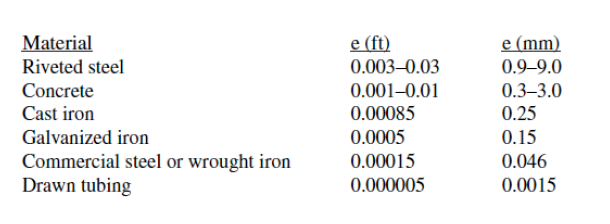
\includegraphics[width=4in]{RoughnessHeights.jpg}
   \caption{Roughness heights for different materials from NCEES Supplied Reference (Moody-Stanton Chart)}
   \label{fig:RoughnessHeights} 
\end{figure}

\item The energy equation for the system is
\begin{equation}
\frac{p_1}{\rho g} + \frac{V_1^2}{2g} + z_1 + h_p = \frac{p_2}{\rho g} + \frac{V_2^2}{2g} + z_2 + h_L
\end{equation}
After substitution of numerical values and the Darcy-Weisbach head loss model, cancellation of identical terms, and isolation of $h_p$, the energy equation is 
\begin{equation}
h_p = 20 + \frac{V^2}{2g}(\frac{f~1000}{10/12} + 0.5 + 1.0)
\end{equation}
\item The system loss for a discharge of 1200, 1600, 2000, 2400, and 2800 gallons-per-minute is shown below in Figure \ref{fig:SystemTable}, which converts the discharges in GPM into CFS, then computes the Reynolds number (viscosity at 60 degrees F was used).  These values were used to enter the Moody chart (Figure \ref{fig:MoodyChart} ) .  The friction factors are all about 0.02 (at our ability to read from the chart).  Once these values are supplied the head loss in the pipeline are computed and used to complete the energy equation.

\begin{figure}[h!] %  figure placement: here, top, bottom, or page
\centering
   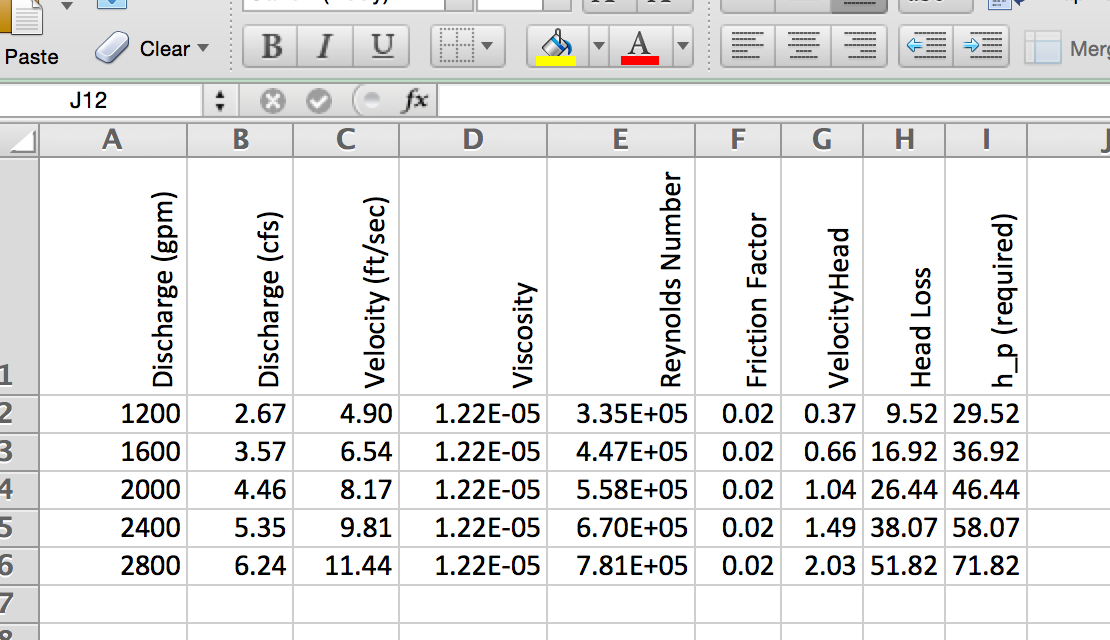
\includegraphics[width=4in]{SystemTable.jpg}
   \caption{Tabulated values for different flow rates in the system.}
   \label{fig:SystemTable} 
\end{figure}

\begin{figure}[h!] %  figure placement: here, top, bottom, or page
\centering
   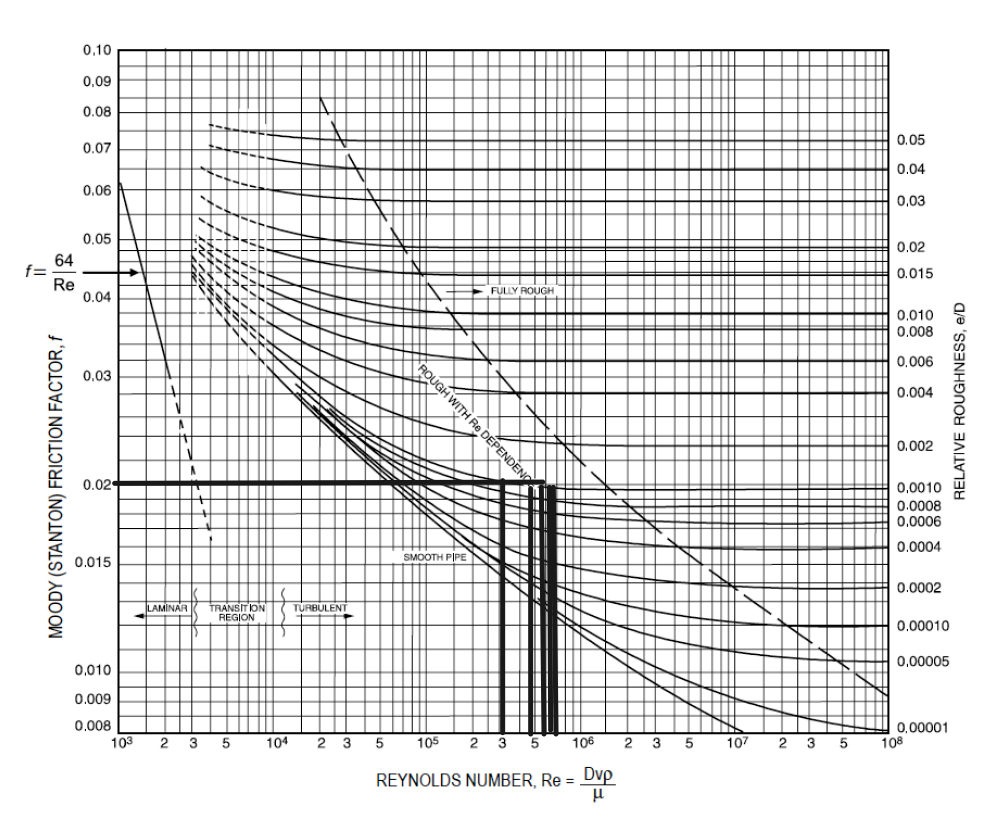
\includegraphics[width=5in]{MoodyChart.jpg}
   \caption{Moody-Stanton Chart}
   \label{fig:MoodyChart} 
\end{figure}

\item The operating discharge for the system using the supplied pump curve is slightly under 2000 gallons-per-minute as shown on \ref{fig:PumpCurve2}.
The point is obtained by plotting the required pump head values from Figure \ref{fig:SystemTable} onto the pump performance curve that was supplied.
\begin{figure}[h!] %  figure placement: here, top, bottom, or page
\centering
   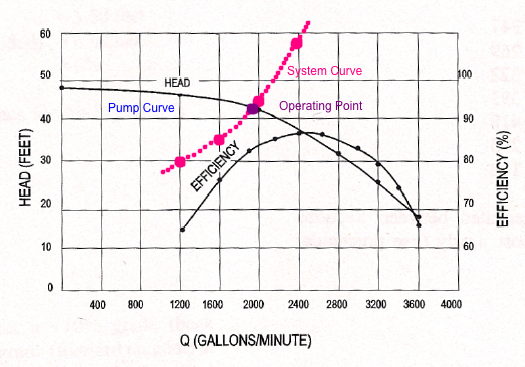
\includegraphics[width=4in]{PumpCurve2.jpg}
   \caption{System and pump characteristic curve on same axes}
   \label{fig:PumpCurve2} 
\end{figure}
\item The electric power supplied to the pump to lift the water at the operating point is
\begin{equation}
P = \frac{Q \rho g h_p}{\eta} = \frac{4.46\times62.4\times46.44}{0.85} = 15,205 \text{~~foot-pounds/second}
\end{equation}
The efficiency value was taken directly from the pump curve and at the operating point, the value of efficiency is about 85-percent.
\\~\\ Conversion to more common units is 
\begin{equation}
15,205 \text{~~foot-pounds/second} \times 1.818\times10^{-3} \times 745.7 = 20,613 \text{~~Watts} = 20.6 \text{kW}
\end{equation}
\end{enumerate}

\section*{\small{Problem 2}}  
This memorandum presents an analysis of a water transfer system that lifts water from one elevation to another.

\section*{\small{Discussion}}
The solution applies the energy equation and pumping concepts, computes a system curve, and uses that curve to find an operating point.
The remainder of this section presents the various steps required, with intermediate calculations shown and references imbedded into the memorandum.
The results for each problem are presented in the narrative below; the by-hand analysis is attached to this memorandum.

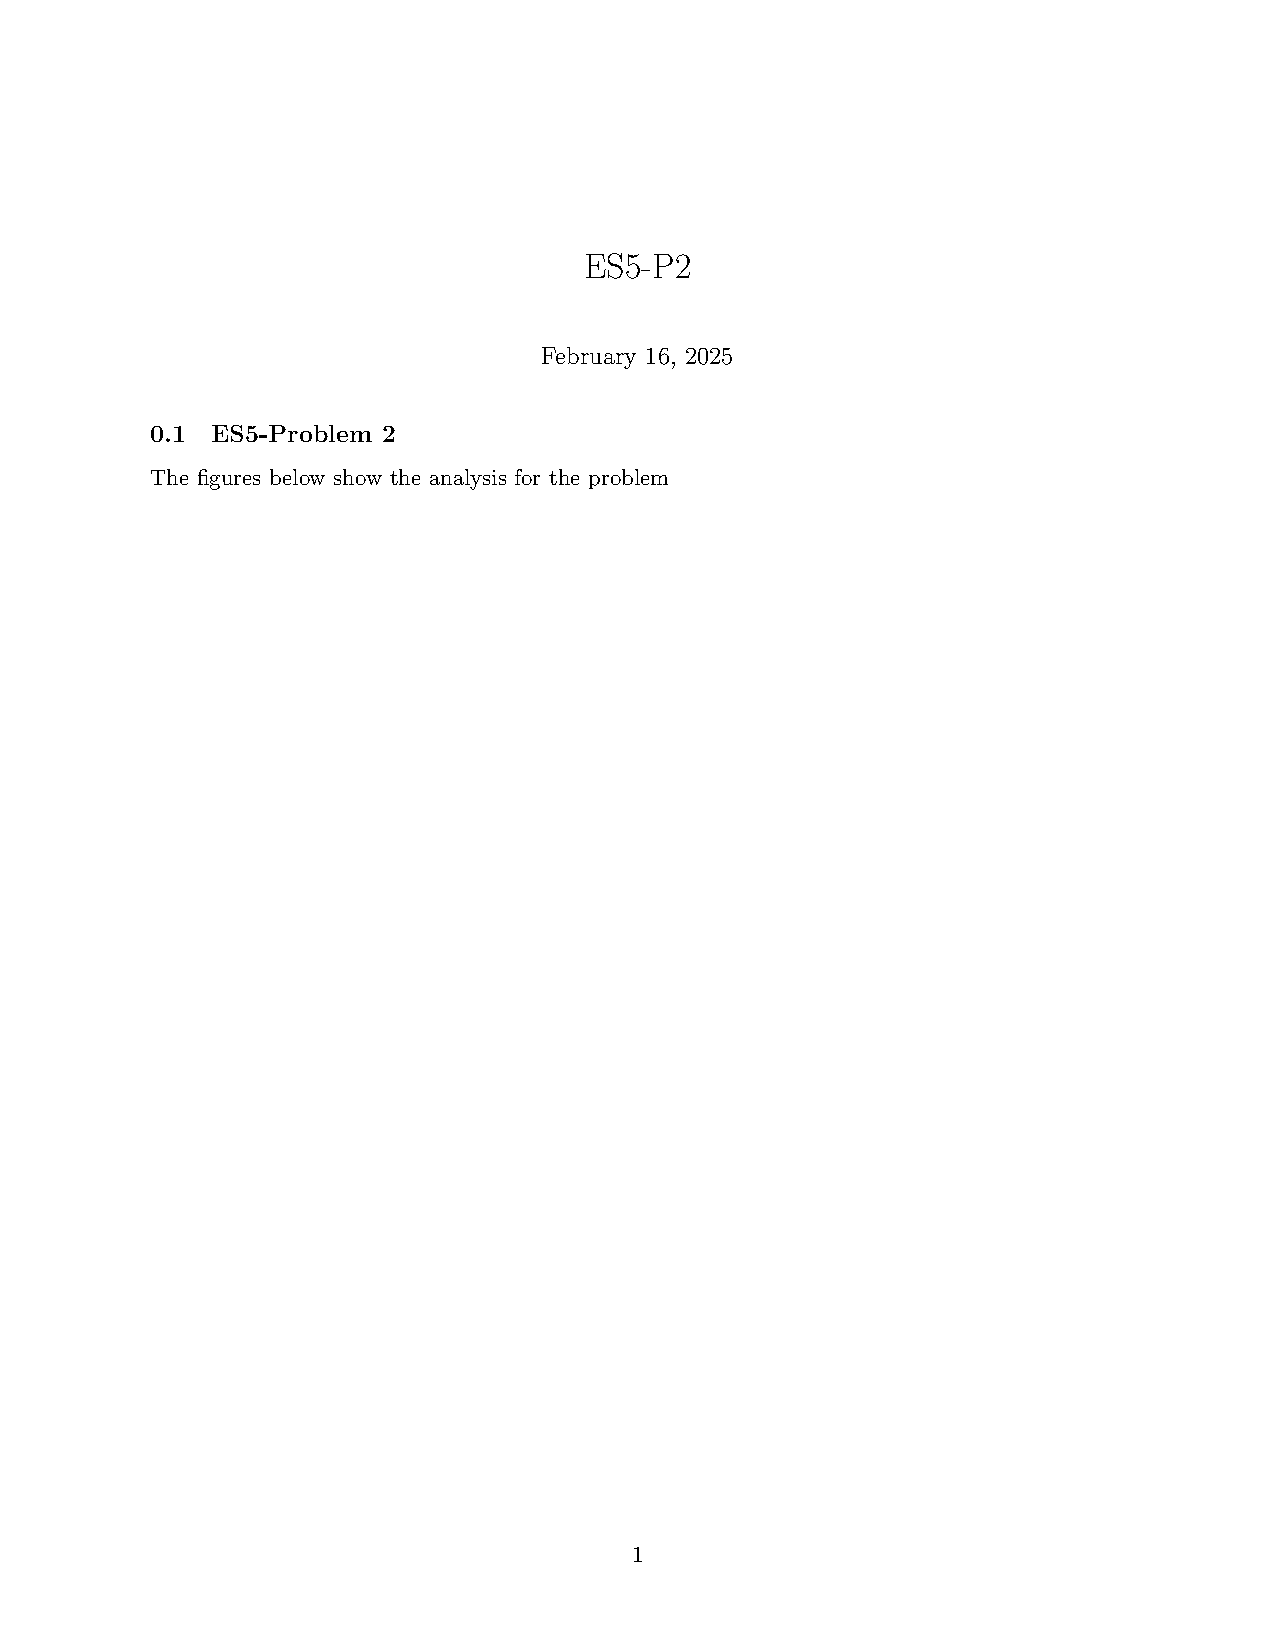
\includepdf[pages={-}]{./ES5-P2.pdf}
%%%%%%%%%%%%%%%%%%%%%%%%%%%%%%%%%%%%%%%%%%%%%%%%%%%%%%%%%%%%%%%%%%%%%%%%%%%%%%
\section*{\small{Conclusion}}
This problems required analysis and application of principles and tools presented in Lecture on Head Loss Models, and Lecture on Pumps.
The use of the Moody chart is enhanced by building the hydraulics calculation table, computing the Reynolds number and looking up the appropriate friction factor.
The entire problem could be done entirely in a spreadsheet if a formula for friction factor was used.   
The particular conditions are along the zero-slope portion of the friction factor curve for the roughness ratio in this case so the friction factor values are essentially the same constant value.

Sincerely, \\
P. Olar Bear \\
Icehaus GmBH \\
\\Attachment(s):\\
None -- entire solution is embedded into the memorandum.

%\begin{thebibliography}{}
%
%\bibitem[\protect\citeauthoryear{Swamee and Jain}{Swamee and Jain}{1976}]{jain1976}
%Swamee and Jain, A. K., 1976. Explicit equations for pipe-flow problems.  ASCE J. of Hyd. Div., 102(HY5) pp. 657-664 
%
%
%\end{thebibliography}


\end{document}  